\documentclass[12pt,openany]{book}
\usepackage{lmodern}
\usepackage{setspace}
\setstretch{1.5}
\usepackage{amssymb,amsmath}
\usepackage{ifxetex,ifluatex}
\usepackage{fixltx2e} % provides \textsubscript
\ifnum 0\ifxetex 1\fi\ifluatex 1\fi=0 % if pdftex
  \usepackage[T1]{fontenc}
  \usepackage[utf8]{inputenc}
\else % if luatex or xelatex
  \ifxetex
    \usepackage{mathspec}
  \else
    \usepackage{fontspec}
  \fi
  \defaultfontfeatures{Ligatures=TeX,Scale=MatchLowercase}
\fi
% use upquote if available, for straight quotes in verbatim environments
\IfFileExists{upquote.sty}{\usepackage{upquote}}{}
% use microtype if available
\IfFileExists{microtype.sty}{%
\usepackage{microtype}
\UseMicrotypeSet[protrusion]{basicmath} % disable protrusion for tt fonts
}{}
\usepackage[left=4cm, right=3cm, top=3cm, bottom=3cm]{geometry}
\usepackage[unicode=true]{hyperref}
\hypersetup{
            pdfborder={0 0 0},
            breaklinks=true}
\urlstyle{same}  % don't use monospace font for urls
\usepackage{longtable,booktabs}
\usepackage{graphicx,grffile}
\makeatletter
\def\maxwidth{\ifdim\Gin@nat@width>\linewidth\linewidth\else\Gin@nat@width\fi}
\def\maxheight{\ifdim\Gin@nat@height>\textheight\textheight\else\Gin@nat@height\fi}
\makeatother
% Scale images if necessary, so that they will not overflow the page
% margins by default, and it is still possible to overwrite the defaults
% using explicit options in \includegraphics[width, height, ...]{}
\setkeys{Gin}{width=\maxwidth,height=\maxheight,keepaspectratio}
\IfFileExists{parskip.sty}{%
\usepackage{parskip}
}{% else
\setlength{\parindent}{0pt}
\setlength{\parskip}{6pt plus 2pt minus 1pt}
}
\setlength{\emergencystretch}{3em}  % prevent overfull lines
\providecommand{\tightlist}{%
  \setlength{\itemsep}{0pt}\setlength{\parskip}{0pt}}
\setcounter{secnumdepth}{5}
\usepackage[none]{hyphenat}
\usepackage[cmyk]{xcolor} % Recommended by US-AB
\usepackage{lmodern} % Recommended by US-AB
\usepackage{fancyhdr}
\usepackage{etoolbox}
\patchcmd{\chapter}{\thispagestyle{plain}}{\thispagestyle{fancy}}{}{} % Removes plain pagestyle from chapter headings (otherwise, page numbers are centered)
\AtBeginDocument{\addtocontents{toc}{\protect\thispagestyle{empty}}} 
\pagestyle{empty} % This makes ToC without header/footer
\usepackage[skip=15pt]{caption} % This should increase space below captions (not tested)
\raggedbottom
\usepackage[noindentafter]{titlesec}
\usepackage{titlesec}
\titleformat{\chapter}{\normalfont\bfseries}{\thechapter.}{15pt}{}\titlespacing*{\chapter}{0pt}{-50pt}{0pt}
\titleformat{\section}{\normalfont\bfseries}{\thesection.}{1em}{}\titlespacing*{\section}{0pt}{0pt}{0pt}
\titleformat{\subsection}[runin]{\normalfont\bfseries}{\thesubsection.}{1em}{}

\usepackage{CJKutf8} % For Mandarin in Acknowledgments

% For guiding quote in beginning of intro:
\makeatletter
% \renewcommand{\@chapapp}{}% Not necessary...
\newenvironment{chapquote}[2][2em]
  {\setlength{\@tempdima}{#1}%
   \def\chapquote@author{#2}%
   \parshape 1 \@tempdima \dimexpr\textwidth-2\@tempdima\relax%
   \itshape}
  {\par\normalfont\hfill--\ \chapquote@author\hspace*{\@tempdima}\par\bigskip}
\makeatother
\usepackage{placeins}
\usepackage{titlesec}

\author{}
\date{\vspace{-2.5em}}

\begin{document}

{
\setcounter{tocdepth}{3}
\tableofcontents
}
\cleardoublepage
\pagestyle{fancy} \fancyhf{} \renewcommand{\headrulewidth}{0pt}
\fancyfoot[LE,RO]{\thepage} \renewcommand{\floatpagefraction}{.9}
\setcounter{page}{9}

\chapter*{Abbreviations}\label{abbreviations}
\addcontentsline{toc}{chapter}{Abbreviations}

\begin{tabular}{ll}
\toprule
Abbreviation & Term\\
\midrule
RPF & Ribosome Protected Fragment\\
\bottomrule
\end{tabular}

\chapter{Introduction}

\section{Cancer}

According to data from the World Cancer Research Fund, in 2018 there
were an estimated 18 million cancer cases worldwide of which 9.5 in men
and 8.5 in women. Lung and breast were the most common cancers overall.
However, the most common cancers among women were breast, colorectal and
lung whereas for men these were lung, prostate and colorectal cancer.

Cancer is a disease in which cells start growing abnormally and evade
mechanisms monitoring cellular integrity. Hanahan et al. (Hanahan \&
Weinberg, 2011) summarised such mechanisms and how cancer evades them as
the hallmarks of cancer. These hallmarks will be discussed in section
xxx.

In this thesis I will discuss two studies in which breast cancer and
pancreatic cancer play a central role. Therefore in the next two
sections will focus on these two very different cancers.

\subsection{Breastcancer}

some text ater the subsection. some more text after the subsection. some
text ater the subsection. some more text after the subsection. some text
ater the subsection. some more text after the subsection.

\subsection{Pancreatic cancer}

stats and explanation on pancreatic cancer

\subsection{Hallmarks of cancer}

Hallmarks of cancer and lead into gene expression

\begin{figure}
  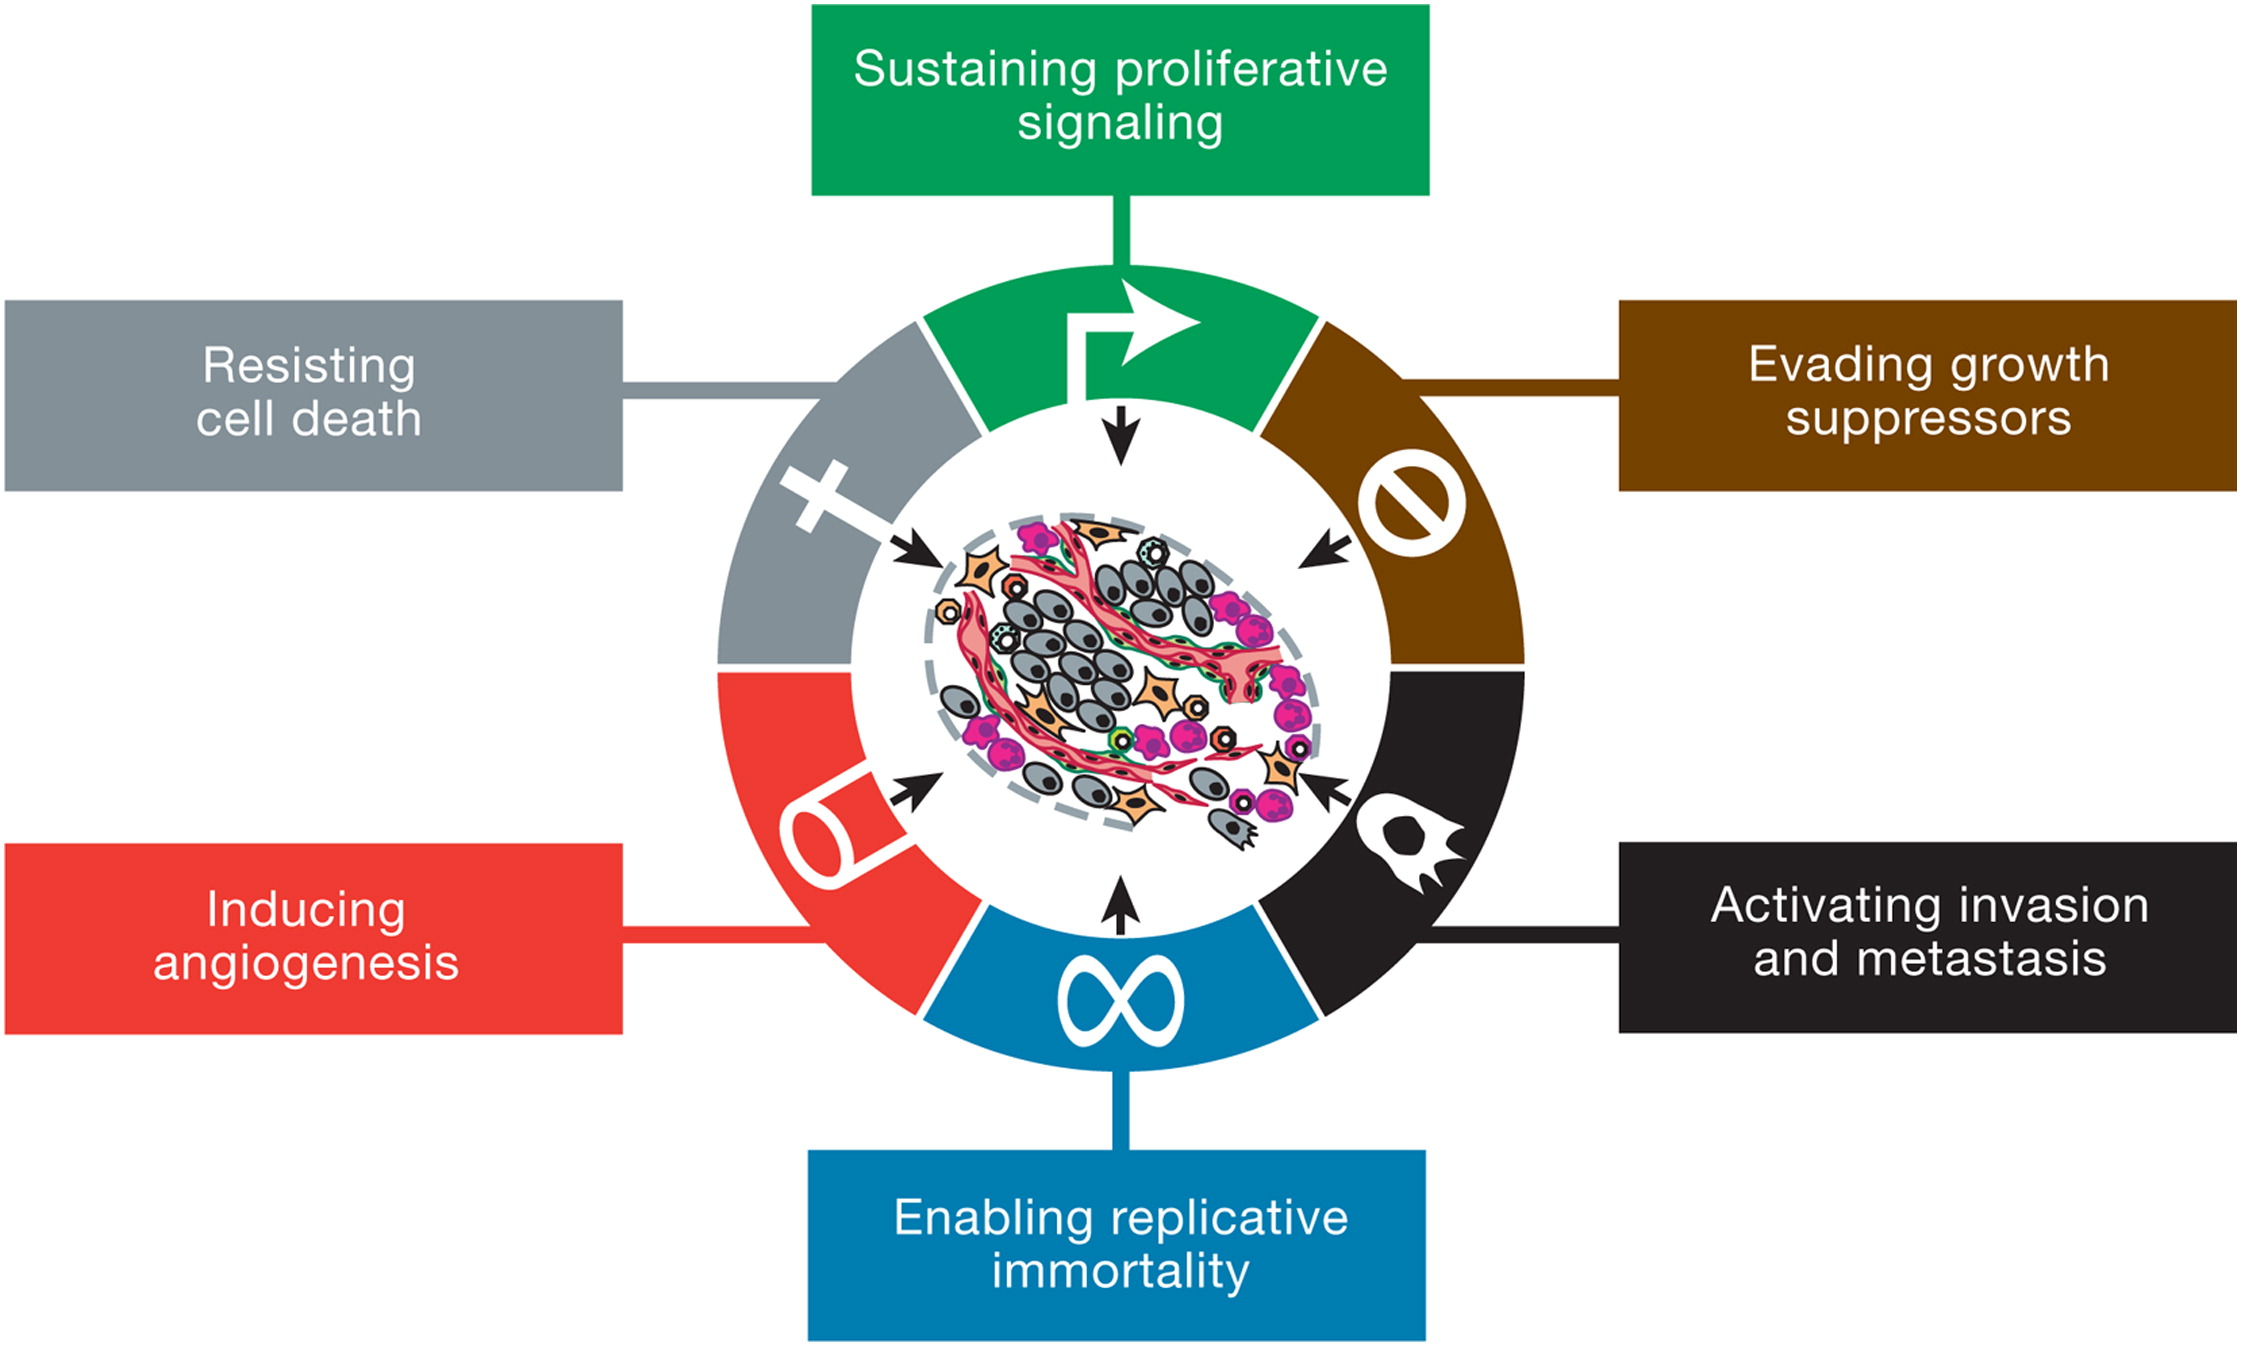
\includegraphics{./figures/hallmarks.jpg}
  \caption{**The Hallmarks of Cancer** - This illustration encompasses the six hallmark capabilities originally proposed in our 2000 perspective. The past decade has witnessed remarkable progress toward understanding the mechanistic underpinnings of each hallmark. Reprinted from Hallmarks of cancer: The next generation, 144, Hanahan, Douglas and Weinberg, Robert A., Hallmarks of cancer: The next generation, 646-674, Copyright (2011), with permission from Elsevier \label{HOC}}
\end{figure}

\section{Central dogma of gene expression}

\section{mRNA translation}

For the vast majority of protein coding mRNAs,eukaryotic mRNA
translation occurs in the cytoplasm, however a small subset of mRNAs is
translated in the mitochondria. mRNA translation is a process that
includes initiation, elongation, termination and ribosome recycling and
is an essential process. mRNA translation inititiation is commonly
regarded as the rate limiting step. Nevertheless, regulation of mRNA
translation is also regulated at the elongation and termination phases
to a lesser extent.

\subsection{mRNA translation initiation}

In eukaryotes most mRNAs are translated by scanning the mRNA for a start
codon (AUG). This mechanism begins with the formation of the 43s
pre-initiation complex (PIC) consisting of methionyl-initiator tRNA
(met-tRNAi) in a ternary complex (TC) with guanosine triphosphate (GTP)
bound eukaryotic initiation factor 2 (eIF2). The PIC is recruited to
the5'-cap of mRNAs which is facilitatedby the eIF4F5'-cap binding
complex, a complex consisting of eIF4E (cap binding protein), eIF4A (RNA
helicase) and eIF4G (scaffolding protein).The PIC then scans along the
mRNA from the 5'end until it encounters an AUG codon. After AUG
recognition eIF2-GTP is hydrolyzed forming a stable 48S PIC.
Afterrelease of eIF2-GTP the 60S ribosomal subunit joins to form the 80S
ribosome and protein synthesis can commence(10, 11). Next to this
scanning mechanism, mRNA translation can also be initiated via
alternative cap independent mechanisms(12).

\subsection{mRNA translation elongation}

The 80S ribosome contains three sites; the acceptor (A), peptidyl (P)
and Exit (E) sites. After initiation, the 80S ribosome is positioned
with the met-tRNAi in the P site at the AUG codon with the following
codon of the transcript in the A site awaiting its cognate tRNA. The
tRNA arrives in a TC together with eukaryotic elongation factor
1A(eEF1A)at the A-site of the ribosome. After arrival in the A-site,the
codon is then recognized. The binding of eEF1A is GTP dependent,
recognition of the cognate codon by the tRNA triggers hydrolysis whereby
eEF1A releases from the tRNA thatis then recycled by eEF1B.Peptide bonds
are then formed accompanied by a tRNA hybrid state whereby acceptor
sites of tRNAs in the A-and P-site now move to the P-and E-site. Binding
of eEF2-GTP then promotes translocation of the tRNAs into the P-and
E-sites after which eEF2B-GDP releases. After release of the deacylated
tRNA from the E-site the ribosome is ready for the next cycle. This
process is repeated until a stop codon (UAA,UGA or UAG)is detected by
the ribosome(11). mRNA translation termination Termination of mRNA
translation is facilitated by two release factors, eRF2 and eRF3-GTP.
The TC with eRF2 and eRF3-GTP binds to the A-site of the ribosome.
Recognition of the stop codon by the ribosome then causes hydrolysis
resulting in a conformational change and release of the polypeptide.
eRF1 and the ATP binding cassette protein (ABCE1) together promote the
splitting of the 60S and 40S subunits, of which the 40S subunits has
still bound tRNA. After release of the tRNA from the 40S subunits the
parts of the translational machinery can be recycled(11).

\section{Regulation of mRNA translation}

\subsection{mTOR singalling pathway}

mTOR is a conserved Ser/Thr kinase and is found in two structurally and
functionally distinct complexes, mTORC1 and mTORC2. mTORC1 contains
mTOR, regulatory associated protein of TOR (raptor), the GTPase
beta-subunit like protein (GbetaL) and disheveled, EGL-10, pleckstrin
{[}DEP{]} domain containing mTOR-interacting protein (deptor). mLST8 and
deptor are found in both mTORC1 and mTORC2.However,
rapamycin-insensitive companion of TOR (rictor), mammalian
stress-activated protein kinase {[}SAPK{]}-interacting protein (mSIN1),
and proline-rich protein 5 (protor) are specific to mTORC2(14, 15). In
regards to regulation of mRNA translation, mTORC1 is a key player in
regulation of translation initiation through facilitating the release of
eIF4E from 4E-BPsvia phosphorylation of 4E-BPs by mTOR (16).
Furthermore, substrates of mTORC1 include ribosomal S6 kinases (S6Ks) 1
and 2(17), and La ribonucleoprotein domain family member 1 (LARP1)(18).
mTORC2 is found to associate with ribosomes to promote co-translational
phosphorylation and foldingofnascent Aktpolypeptide(19).As mentioned
mTORC1 is activated via growth hormonesincludinginsulin and insulin like
growth factor (IGF).For example,wheninsulin binds to the insulin
receptor,tyrosine kinases (RTKs) and phosphoinositide 3-kinase (PI3K)
are activated. Phosphatidylinositol 3,4,5-triphosphate (PIP3) is then
generated by PI3K from Phosphatidylinositol 4,5-biphoasphate (PIP2).
This step is reversed by PTEN which hydrolyzes PIP3 to PIP2, thereby
working antagonistically to PI3K. PIP3 recruits AKT and
phosphoinositide-dependent kinase1 (PDK1) towards the plasma membrane
where AKT is phosphorylated by PDK1. Ras homologue enriched in brain
(Rheb) is a GTPase that stimulates mTOR in its GTP bound form. The
tuberous sclerosis complex (TSC) consists of TSC1 (scaffold protein) and
TSC2 is a GTPase-activating protein (GAP) which inhibits Rheb through
hydrolysis of Rheb-GTP to Rheb-GDP, thereby inhibiting mTOR activity.
AKT mediates phosphorylation of TSC2, leading to a decreased GAP
activity and reduced mTOR inhibition. Signaling through the Ras GTPase
by growth factors may also activate mTORC1 through the RAF/MEK/ERK axis
whereby extracellular signal-regulated kinase (ERK) leads to direct
phosphorylation of TSC2 and raptor or via the RSKs(6, 20, 21).Protein
synthesis is the most energy expensive process within
cells(22).Therefore,regulation of mRNA translation is tied to cellular
energy levels. AMP-activated protein kinase (AMPK) is a kinase activated
by increased AMP/ATPratioas well as ADP/ATP ratios. AMPK inhibits
protein synthesis by activation of TSC2, thereby reducing mTOR activity.
Furthermore, cellular oxygen levels are linked to ATP production, where
low oxygen levels reduce ATP production leading to AMPK
activation(23).mTOR modulates global mRNA translation mainly
throughmodulation of 4E-BPs and S6Ks(24, 25). However,mTOR also mediates
selectivemRNA translation (26). Upon activation, mTORphosphorylates
4E-BPsleading to release of eIF4E(6, 14). As described above eIF4E then
facilitates assembly of eIF4F, whichis essential for cap dependent mRNA
translation initiation. S6Ks (S6K1 and S6K2) phosphorylates multiple
componentof the translational machinery such as RPS6which is implicated
in ribosome biogenesis(27). Furthermore, S6Ks also phosphorylateeEF2
kinase which is a negative regulator of protein synthesis(28).Lastly,
S6Ks phosphorylate programmed cell death 4 (PDCD4)triggering its
SCFbetaTrCP-dependent degradation (29).PDCD4is a factor blocking the
eIF4A-eIF4G interactionby binding to eIF4A.Binding of PDCD4 to eIF4A
leads to inhibitionof eIF4A activity and thus translation of mRNAsthat
require RNA helicase activity(30). More recent work indicates an effect
of mTORC1on LA motif (LAM)-containing factor family La-related protein 1
(LARP1). In that study theconserved RNA-binding protein of
LARP1interacts with raptor and is phosphorylated by mTORC1.However, the
scope of LARP1 mediated effectsremaincontroversial.It has been suggested
LARP1 stabilizes or regulates translation of mRNAs with the terminal
oligo pyrimidine (TOP) motif in a context dependent manner(18, 31, 32).

\chapter{Aims of this thesis}

The aims of this thesis are to explore the regulation of gene expression
in cancer, more specifically we investigate perturbations of gene
expression in different cancer models as a response to drug treatment.

In \textbf{Study I} we adapted an algorithm for ANalysis Of Translation
Activity data (anota) so that it could be applied to next generation
sequencing data. The resulting algorithm was named anota2seq.

We then applied the anota2seq algortihm to invesitigate changes in
translation efficiencies in two cancer models:

In \textbf{Study II} we unravelled the effects of eIF4A, an RNA
helicase, inhibition using a synthetic rocaglate CR-1-31-B (CR-31) in
pancreatic ductal adenocarcinoma.

In \textbf{Study III} we explored the effects of insulin on gene
expression in a breast cancer cell line.

\chapter{Results and discussion}

\chapter{Conclusions}

\chapter*{Acknowledgments}\label{acknowledgments}
\addcontentsline{toc}{chapter}{Acknowledgments}

Christina is awesome.

I am sorry for all the other people of this page but no one else helped
me more than my 8 paws of awesomeness Felix and Dexter. These little
litter shitters have been an extreme joy to be around and kept me sane
during the insanity that is writing a thesis. \textbf{Meow}

\chapter*{References}\label{references}
\addcontentsline{toc}{chapter}{References}

\hypertarget{refs}{}
\hypertarget{ref-Hanahan2011}{}
Hanahan, D., \& Weinberg, R. A. (2011). Hallmarks of cancer: The next
generation. \emph{Cell}, \emph{144}(5), 646--674.
\url{https://doi.org/10.1016/j.cell.2011.02.013}

\end{document}
